\documentclass{article}

\usepackage[utf8]{inputenc} % Required for inputting international characters
\usepackage[T1]{fontenc} % Output font encoding for international characters
\usepackage[backend=bibtex,style=alphabetic,natbib=true]{biblatex}
\addbibresource{references.bib}
\usepackage{amsmath, amssymb, amsfonts, amsthm, stmaryrd}
\usepackage{caption}
\usepackage{subcaption}
\usepackage{graphicx}
\usepackage{enumitem}
\usepackage{mathpartir}
\usepackage{bussproofs}
\usepackage{xparse}
\usepackage[usenames, dvipsnames]{xcolor}
\usepackage{lipsum}
\usepackage{xargs}
\usepackage{hyperref}
\usepackage{tikz-cd}
\usepackage{todonotes}
\usepackage{url}
\usepackage{xspace}
\usepackage{rotating}
\usepackage{quiver}
\usepackage[backend=bibtex,style=alphabetic,natbib=true]{biblatex}
\addbibresource{references.bib}
\usepackage{array}   % for \newcolumntype macro
\newcolumntype{C}{>{$}c<{$}} % math-mode version of "l" column type
\newcolumntype{L}{>{$}l<{$}} % math-mode version of "l" column type

% \usepackage{draftwatermark}
% \SetWatermarkText{Confidential}
% \SetWatermarkScale{4}
% \SetWatermarkColor[gray]{0.9}

\hypersetup{
  linktocpage,
  colorlinks,
  citecolor=BlueViolet,
  filecolor=red,
  linkcolor=Blue,
  urlcolor=BrickRed
}
\newcommand{\mpav}[1]{\textcolor{red}{\textsc{Marco}: #1}}
\newcommand{\proofcomment}[1]{\text{\{ #1 \}}}
\newenvironment{proofof}[1] {\begin{proof}[Proof of {#1}]}{\end{proof}}
\newcommand{\eqdef}{\stackrel{\mathrm{\Delta}}{=}}
\newcommand{\bnfeq}{\mathrel{::=}}
\newcommand{\defeq}{\triangleq}
\newcommand{\rul}[3]{\frac{#2}{#3}\;  {\textrulelabel{#1}}}
\newcommand{\den}[1]{\llbracket #1 \rrbracket}
\newcommand{\jud}[3]{#1 \vdash #2 : #3}
\newcommand{\bden}[1]{\llparenthesis#1 \rrparenthesis}
\newcommand{\bigslant}[2]{{\raisebox{.2em}{$#1$}\left/\raisebox{-.2em}{$#2$}\right.}}
\newcommand{\quotient}[2]{\bigslant{#1}{#2}}

\newcommand{\curry}{\Lambda}
\newcommand{\uncurry}{\begin{sideways}\begin{sideways}$\Lambda$\end{sideways}\end{sideways}}

\newcommand{\Bool}{\mathbb{B}}
\newcommand{\N}{\mathbb{N}}
\newcommand{\Nat}{\N}
\newcommand{\Sets}{\mathbf{Set}}
\newcommand{\blacklater}{\blacktriangleright}
\newcommand{\tot}{\mathcal{S}}
\newcommand{\PSh}{\ensuremath{\textbf{PSh}(\omega)}}

\newsavebox{\lbananabox}
\newcommand{\lbananamacro}{%
  
\begin{tikzpicture}[baseline=0.25em,xscale=0.005em,yscale=0.005em]
  \draw[solid, join=round] (2,0) to[out=140,in=-90] (0,3) to[out=90,in=-140] (2,6) -- (2.1,5.9)
              to[out=-120,in=90] (1.2,3) to[out=-90,in=120] (2.1,0.1) -- cycle;
\end{tikzpicture}
}
\savebox{\lbananabox}{\lbananamacro}
\newcommand{\lbanana}{\mathopen{\usebox{\lbananabox}\hspace{-0.6ex}}}


\newsavebox{\rbananabox}
\newcommand{\rbananamacro}{%
  
\begin{tikzpicture}[baseline=0.25em,xscale=-0.005em,yscale=0.005em]
  \draw[solid, join=round] (2,0) to[out=140,in=-90] (0,3) to[out=90,in=-140] (2,6) -- (2.1,5.9)
              to[out=-120,in=90] (1.2,3) to[out=-90,in=120] (2.1,0.1) -- cycle;
  \end{tikzpicture}
}
\savebox{\rbananabox}{\rbananamacro}
\newcommand{\rbanana}{\mathclose{\usebox{\rbananabox}}}


\newsavebox{\lbansbox}
\newcommand{\lbansmacro}{%
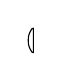
\begin{tikzpicture}[baseline=0.45ex,xscale=0.006em,yscale=0.012ex]%
% curvey bananas
%\draw[solid,join=round,fill=yellow] (2,0) to[out=140,in=-90] (0,3) to[out=90,in=-140] (2,6) -- (2.1,5.9) to[out=-120,in=90] (1.2,3) to[out=-90,in=120] (2.1,0.1) -- cycle;%
% fitted lenses
\draw[solid,join=round] (1.8,6) -- (1.5,5.9) to[out=-120, in=90] (0.7,3) to[out=-90, in=120] (1.5,0.1) -- (1.8,0) -- cycle;%
\end{tikzpicture}}
\savebox{\lbansbox}{\lbansmacro}
\newcommand{\lbans}{\mathopen{\usebox{\lbansbox}\mspace{1mu}}}

\newsavebox{\rbansbox}
\newcommand{\rbansmacro}{%
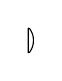
\begin{tikzpicture}[baseline=0.45ex,xscale=-0.006em,yscale=0.012ex]%
% curvey bananas
%\draw[solid,join=round,fill=yellow] (2,0) to[out=140,in=-90] (0,3) to[out=90,in=-140] (2,6) -- (2.1,5.9) to[out=-120,in=90] (1.2,3) to[out=-90,in=120] (2.1,0.1) -- cycle;%
% fitted lenses
\draw[solid,join=round] (1.8,6) -- (1.5,5.9) to[out=-120, in=90] (0.7,3) to[out=-90, in=120] (1.5,0.1) -- (1.8,0) -- cycle;%
\end{tikzpicture}}
\savebox{\rbansbox}{\rbansmacro}
\newcommand{\rbans}{\mathclose{\mspace{1mu}\usebox{\rbansbox}}}

\newsavebox{\llensbox}
\newcommand{\llensmacro}{%

\begin{tikzpicture}[baseline=0.45ex,xscale=0.006em,yscale=0.012ex]%
\draw[solid,join=round] (1.4,0) -- (0,0) -- (0,6) -- (1.4,6) -- (1.5,5.9) to[out=-120, in=90] (0.7,3) to[out=-90, in=120] (1.5,0.1) -- cycle;%
\end{tikzpicture}}
\savebox{\llensbox}{\llensmacro}
\newcommand{\llens}{\mathopen{\usebox{\llensbox}\mspace{1mu}}}

\newsavebox{\rlensbox}
\newcommand{\rlensmacro}{%
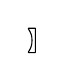
\begin{tikzpicture}[baseline=0.45ex,xscale=-0.006em,yscale=0.012ex]%
\draw[solid,join=round] (1.4,0) -- (0,0) -- (0,6) -- (1.4,6) -- (1.5,5.9) to[out=-120, in=90] (0.7,3) to[out=-90, in=120] (1.5,0.1) -- cycle;%
\end{tikzpicture}}
\savebox{\rlensbox}{\rlensmacro}
\newcommand{\rlens}{\mathclose{\mspace{1mu}\usebox{\rlensbox}}}

% filled versions
\newcommand{\Lbanana}{%
  \mathopen{\mspace{1mu}\tikz[baseline=0.25em,xscale=0.006em,yscale=0.006em]
  \fill (2,0) to[out=140,in=-90] (0,3) to[out=90,in=-140] (2,6) -- (2.1,5.9)
              to[out=-120,in=90] (1.2,3) to[out=-90,in=120] (2.1,0.1) -- cycle;\mspace{1mu}}}
\newcommand{\Rbanana}{%
  \mathclose{\mspace{1mu}\tikz[baseline=0.25em,xscale=-0.006em,yscale=0.006em]
  \fill (2,0) to[out=140,in=-90] (0,3) to[out=90,in=-140] (2,6) -- (2.1,5.9)
              to[out=-120,in=90] (1.2,3) to[out=-90,in=120] (2.1,0.1) -- cycle;}}
% % lens brackets (using TikZ)
% \newcommand{\llens}{%
%   \mathopen{\tikz[baseline=0.25em,xscale=0.006em,yscale=0.006em]
%   \draw[join=round] (1.4,0) -- (0,0) -- (0,6) -- (1.4,6) -- (1.5,5.9)
%         to[out=-120,in=90] (0.7,3) to[out=-90,in=120] (1.5,0.1) -- cycle;\mspace{1mu}}}
% \newcommand{\rlens}{%
%   \mathclose{\mspace{1mu}\tikz[baseline=0.25em,xscale=-0.006em,yscale=0.006em]
%   \draw[join=round] (1.4,0) -- (0,0) -- (0,6) -- (1.4,6) -- (1.5,5.9)
%         to[out=-120,in=90] (0.7,3) to[out=-90,in=120] (1.5,0.1) -- cycle;}}
% filled versions
\newcommand{\Llens}{%
  \mathopen{\tikz[baseline=0.25em,xscale=0.006em,yscale=0.006em]
  \fill (1.4,0) -- (0,0) -- (0,6) -- (1.4,6) -- (1.5,5.9)
        to[out=-120,in=90] (0.7,3) to[out=-90,in=120] (1.5,0.1) -- cycle;\mspace{1mu}}}
\newcommand{\Rlens}{%
  \mathclose{\mspace{1mu}\tikz[baseline=0.25em,xscale=-0.006em,yscale=0.006em]
  \fill (1.4,0) -- (0,0) -- (0,6) -- (1.4,6) -- (1.5,5.9)
        to[out=-120,in=90] (0.7,3) to[out=-90,in=120] (1.5,0.1) -- cycle;}}


\newcommand{\anamor}[1]{{\llens\, #1\, \rlens}}
\newcommand{\catamor}[1]{\lbans\, #1\, \rbans}
\newcommand{\cata}[1]{\lbans #1 \rbans}
\newcommand{\ana}[1]{\llens #1 \rlens}
\newcommand{\fold}[1]{\catamor{#1}}
\newcommand{\unfold}[1]{\anamor{#1}}

\newcommand{\operator}[1]{\textsf{#1}}
\newcommand{\Alg}{\text{-Alg}}
\newcommand{\Free}{\text{Free\xspace}}

\newcommand{\CatC}{\mathcal{C}}
\newcommand{\CatD}{\mathcal{D}}
\newcommand{\CatE}{\mathcal{E}}
\newcommand{\CatI}{\mathcal{I}}

\newcommand{\Set}{\mathbf{Set}}
\newcommand{\iso}{\cong}
\newcommand{\ceiling}[1]{\lceil #1 \rceil}
\newcommand{\floor}[1]{\lfloor #1 \rfloor}

\newcommand{\pair}[2]{\langle #1, #2 \rangle}
\newcommand{\InIso}{\text{In}}

\title{Hylomorphisms in Coq}

\author{}

\begin{document}

\maketitle

\section{Adjoint Folds}

\subsection{Canonical Adjoint Folds}
\[\begin{tikzcd}
	{\CatC} & \CatD
	\arrow[""{name=0, anchor=center, inner sep=0}, "L"', shift right=2, from=1-2, to=1-1]
	\arrow[""{name=1, anchor=center, inner sep=0}, "R"', shift right=2, from=1-1, to=1-2]
	\arrow["\dashv"{anchor=center, rotate=-90}, draw=none, from=0, to=1]
    \arrow["D"', loop, distance=2em, in=35, out=325, from=1-2, to=1-2]
    \arrow["LDR"', loop, distance=2em, in=215, out=145, from=1-1, to=1-1]
\end{tikzcd}
\]

The following is a natural isomorphism arising from the adjunction $L \dashv R$.
\begin{equation}
  \label{eq:adjoint-iso}
  \floor{\cdot} : \CatC(LA, B) \iso \CatD (A, RB) : \ceiling{\cdot}
\end{equation}
Some properties of adjunctions are worth recalling.  The unit and counit of the
adjunction can be defined from the above isomorphism as follows:
\[
  \eta_{A} = \floor{id_{LA}} \qquad \epsilon_{B}  = \ceiling{id_{RB}}
\]
Conversely, the isomorphism can be defined in terms of the two functors $L$ and
$R$ and the units of the adjunction:
\begin{align*}
  & \floor{f : LA \to B} = A \xrightarrow{\eta_{A}} RLA \xrightarrow{R(f)} RB\\
  & \ceiling{g : A \to RB} = LA \xrightarrow{L(g)} LRB \xrightarrow{\epsilon_{B}} B
\end{align*}
These definitions are going to be useful later to understand the definitions of
the recursion schemes we are going to prove correct.

As a result, the following two diagrams (recursion schemes) are equivalent. The
on the right hand side is a \emph{catamorphism} taking a $D$ algebra on $RB$ and
construting an inductive function over the data type $\mu D$. The one on the
left hand side is the derived recursion scheme where the data type has been
wrapped up in $L$. The transformation is done by just applying the isomorphism
(\ref{eq:adjoint-iso}) given by the adjunction.

\begin{equation}
  \label{eq:canonical-adjoint-fold}
  \begin{tikzcd}
	{LD\mu D} & LDRB && {D\mu D} & DRB \\
	{L\mu D} & B & {} & {\mu D} & RB
	\arrow["{\cata{a}}"', from=2-4, to=2-5]
	\arrow[""{name=0, anchor=center, inner sep=0}, "{\InIso}"', from=1-4, to=2-4]
	\arrow["{D(\cata{a})}", from=1-4, to=1-5]
	\arrow["{\floor{a}}", from=1-5, to=2-5]
	\arrow["{\ceiling{\cata{a}}}"', from=2-1, to=2-2]
	\arrow["{L(\InIso)}"', from=1-1, to=2-1]
	\arrow["{LD(\cata{a})}", from=1-1, to=1-2]
	\arrow[""{name=1, anchor=center, inner sep=0}, "a", from=1-2, to=2-2]
	\arrow[shorten <=28pt, shorten >=28pt, Rightarrow, 2tail reversed, from=1, to=0]
  \end{tikzcd}
\end{equation}

In the following section we instantiate the adjoint fold with some instances
taken from the literature.

\subsection{Example}
Say that we want to prove that the two functions below are well-defined

\begin{tabular}{LL}
  \operator{even} : \Nat \to \Bool                  &  \operator{odd} : \Nat \to \Bool\\
  \operator{even} (0) = \top                        &  \operator{odd}(0) = \top\\
  \operator{even} (n+1) = \neg \operator{odd}(n)    &  \operator{odd}(n+1) = \neg (\operator{even}(n))
\end{tabular}

One option is to prove that the following function (given by a catamorphism) is
equivalent to the above
\begin{align*}
  & \operator{even-odd} : \Nat \to \Bool \times \Bool\\
  & \operator{even-odd} (0) = (\top, \bot)\\
  & \operator{even-odd} (n+1) = \operator{let } (x,y) \leftarrow \operator{even-odd}(n) \operator{ in } (\neg x, \neg y)
\end{align*}
This function is clearly a catarmorphism:
\begin{align*}
  & \operator{even-odd} : \Nat \to \Bool \times \Bool\\
  & \operator{even-odd} = \cata{a} \operator{ where }\\
  & \qquad \qquad a : 1 + (\Bool \times \Bool)\\
  & \qquad \qquad a (\operator{nil}) = (\top, \bot)\\
  & \qquad \qquad a (\operator{x,y}) = (\neg x, \neg y)
\end{align*}
where $\cata{\cdot}$ takes a $(1+-)$ algebra on $\Bool \times \Bool$ and returns
the associated recursive function.

In order to transform $\operator{even-odd}$ into two functions $\operator{even}$
and $\operator{odd}$ we are going to use the adjunction $\Delta \vdash \times$
where $\Delta : \CatC \to \CatC \times \CatC$ is the diagonal functor
$\Delta X = (X,X)$ and $\times : \CatC \times \CatC$ is the product seen as a
bifunctor

\[\begin{tikzcd}
	{\CatC \times \CatC} & \CatC
	\arrow[""{name=0, anchor=center, inner sep=0}, "\Delta"', shift right=2, from=1-2, to=1-1]
	\arrow[""{name=1, anchor=center, inner sep=0}, "\times"', shift right=2, from=1-1, to=1-2]
	\arrow["\dashv"{anchor=center, rotate=-90}, draw=none, from=0, to=1]
    \arrow["D"', loop, distance=2em, in=35, out=325, from=1-2, to=1-2]
    \arrow["\Delta\circ D\circ \times "', loop, distance=2em, in=215, out=145, from=1-1, to=1-1]
\end{tikzcd}
\]
To get the natural isomorphism from this adjunction we can instantiate
(\ref{eq:adjoint-iso}) as follows
\[
  \floor{\cdot} : \CatC \times \CatC ((A, A) , (B_{1}, B_{2}) \iso \CatC (A , B_{1} \times B_{2}): \ceiling{\cdot}
\]
We can instantiate further the iso by setting $A = \Nat$, $B_{1} = \Bool$ and
$B_{2} = \Bool$.
\[
  \floor{\cdot}: \CatC \times \CatC ((\Nat, \Nat) , (\Bool, \Bool) \iso \CatC (\Nat , \Bool \times \Bool) : \ceiling{\cdot}
\]

To define this isomorphism we can just define the units of the adjunctions:
\begin{align*}
  & \eta_{A} : A \to A \times A\\
  & \eta_{A}= \pair{id_{A}}{id_{a}}\\
  & \epsilon_{(X,Y)} : ((X \times Y), (X \times Y) \to (X,Y)\\
  & \epsilon_{(X,Y)} = (\pi_{1}, \pi_{2})
\end{align*}
Notice that, in particular, the counit is given by the projections out of the
product.  Now, the right transponse $\ceiling{\cdot}$ of the adjunction can be
defined using the projections provided by the counit.  And in fact, the ceiling
can be defined as
\[
  \ceiling{g} = (\pi_{1},\pi_{2}) \cdot \Delta(g) =  (\pi_{1},\pi_{2}) \cdot (g,g) = (\pi_{1} \cdot g,\pi_{2}\cdot g)
\]
and the floor can be defined as
\[
  \floor{f}(a) = \pair{f(a)}{f(a)}
\]
At this point we are pretty much done as we can instantiate the diagrams
(\ref{eq:canonical-adjoint-fold}) where $D X = 1 + X$
\[
  \begin{tikzcd}
	{(1 + \Nat, 1 + \Nat)} && (1 + \Bool \times \Bool, 1 + \Bool \times \Bool) & { 1 + \Nat} & 1 + (\Bool \times \Bool) \\
	{(\Nat, \Nat)} && (\Bool, \Bool) & {\Nat} & \Bool \times \Bool
	\arrow["{\cata{a}}"', from=2-4, to=2-5]
	\arrow[""{name=0, anchor=center, inner sep=0}, "{\InIso}"', from=1-4, to=2-4]
	\arrow["{1 + \cata{a}}", from=1-4, to=1-5]
	\arrow["a", from=1-5, to=2-5]
	\arrow["{\ceiling{\cata{a}}}"', from=2-1, to=2-3]
	\arrow["{(1 +  \InIso,1 +  \InIso)}"', from=1-1, to=2-1]
	\arrow["{(1 + \cata{a}, 1 + \cata{a})}", from=1-1, to=1-3]
	\arrow[""{name=1, anchor=center, inner sep=0}, "\ceiling{a}", from=1-3, to=2-3]
	\arrow[shorten <=35pt, shorten >=35pt, Rightarrow, 2tail reversed, from=1, to=0]
  \end{tikzcd}
\]
Now we define $a$ to be the following $D$ algebra:
\begin{align*}
  & a : 1 + \Bool \times \Bool \to \Bool\\
  & a (\operator{nil}) = (\top, \bot)\\
  & a (b_{1}, b_{2}) = (\neg b_{1}, \neg b_{2})
\end{align*}

It is easy to see that the catamorphism over the algebra $a$ equals
$\operator{even-odd}$ and by the adjoint fold property we know that its right
transpose satisfies the right hand side diagram. We now have to show that the
pair of functions $(\operator{even}, \operator{odd})$ equals the right transpose
of $\operator{even-odd}$, but this is easy to see by definition of the ceiling:
\[
  \ceiling{\operator{even-odd}} = (\pi_{1}\cdot \operator{even-odd}, \pi_{2}\cdot \operator{even-odd})
\]
and then it is an easy calculation to see that $\pi_{1}\cdot \operator{even-odd}$ equals $\operator{even}$ and
that $\pi_{2}\cdot \operator{even-odd}$ equals $\operator{odd}$.
\end{document}
